\documentclass{article}
\usepackage{leonine,amsmath,amssymb,amsthm,graphicx,algorithm,algorithmic}
\setkeys{Gin}{width=\linewidth,totalheight=\textheight,keepaspectratio}
\graphicspath{{graphics/}}
% Prints a trailing space in a smart way.
\usepackage{xspace}
% Inserts a blank page
\newcommand{\blankpage}{\newpage\hbox{}\thispagestyle{empty}\newpage}
% \usepackage{units}
% Typesets the font size, leading, and measure in the form of 10/12x26 pc.
\newcommand{\measure}[3]{#1/#2$\times$\unit[#3]{pc}}

\theoremstyle{definition}
\newtheorem{pred}[thm]{Prediction}

\def\ent{=\joinrel\mathrel|}

\title{Cerebellum} \author{Eric Purdy}

\begin{document}

\maketitle

\section{Overview}

We posit that the cerebellum as a whole tries to predict the output of
the cerebrum, and takes over the performance of activities that are
sufficiently predictable. Ito \cite{ito} posits a similar theory
(specifically, the inverse models from his paper).

\begin{figure}
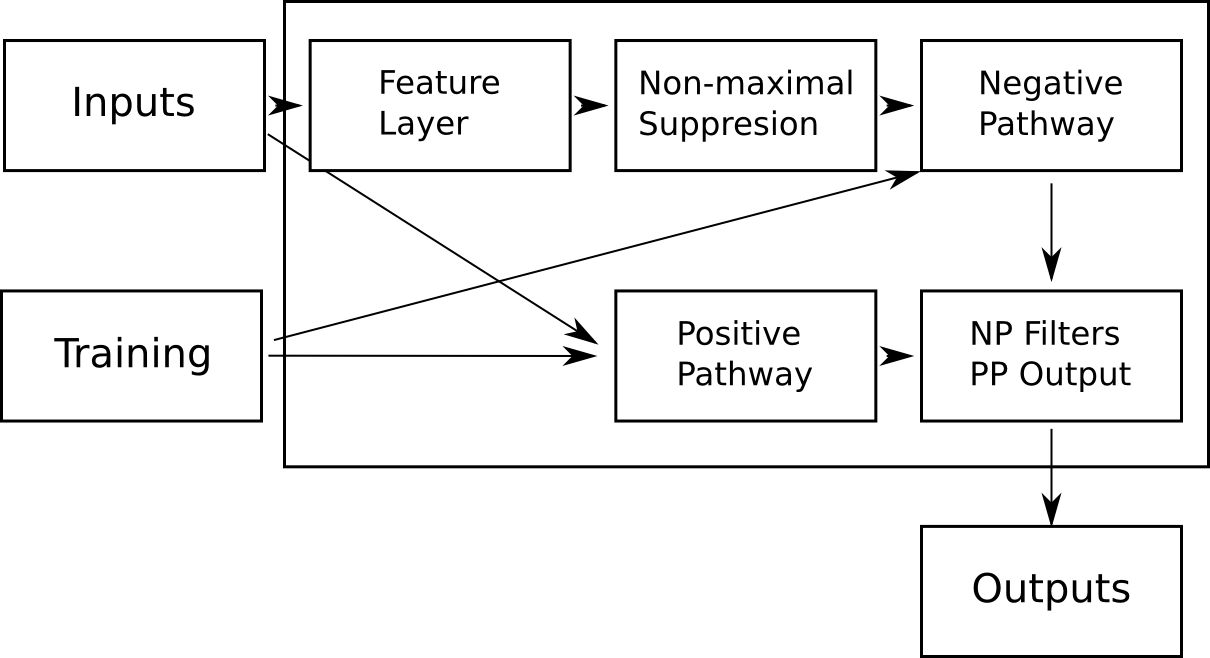
\includegraphics[width=\linewidth]{computation.png}
\caption{Computations performed by the cerebellum}
\label{fig-computation}
\end{figure}

\begin{algorithm}
\caption{$cerebellum(\mathbf{command}^{(t-1)},\mathbf{context}^{(t-1)}, \mathbf{train}^{(t-1)})$}
\begin{algorithmic}
  \FNSTATE $\mathbf{state}^{(t-1)}$

  \FOR{$i = 0$ to $n$}
  \STATE{$\mathbf{pos\_state}_i^{(t)} \from positive\_state\left(\mathbf{state}^{(t-1)}, \mathbf{command}^{(t-1)}, \mathbf{context}^{(t-1)} \right)$}
  \ENDFOR
  \FOR{$j = 0$ to $m$}
  \STATE{$\mathbf{pos\_output}_j^{(t)} \from positive\_output\left(\mathbf{state}^{(t-1)}, \mathbf{command}^{(t-1)}, \mathbf{context}^{(t-1)} \right)$}
  \ENDFOR

  \COMMENT{Compute simple features}
  \FOR{$k = 0$ to $K$}
  \STATE{$\mathbf{feat}_k^{(t)} \from feature\_layer\left( \right)$}
  \ENDFOR

  \COMMENT{For each cluster of features, compute average activation}
  \FOR{$l = 0$ to $L$}
  \STATE{$\mathbf{cluster\_avg} \from cluster\_avg\left( \right)$}
  \ENDFOR
  
  \COMMENT{All cluster elements are lessened by the cluster average}
  \FOR{$k = 0$ to $K$}
  \STATE{$\mathbf{feat\_nms}_k^{(t)} \from subtract\_avg\left(
    \mathbf{feat}_k^{(t)}, 
    \mathbf{cluster\_avg}_l^{(t)}\right)$}
  \ENDFOR
  
  \COMMENT{Negative pathway is a collection of perceptrons on $\mathbf{feat\_nms}$}
  \FOR{$p = 0$ to $P$}
  \STATE{$\mathbf{neg\_output}_p^{(t)} \from negative\_output\left(
    \mathbf{feat\_nms}^{(t)}\right)$}
  \ENDFOR

  \COMMENT{Negative pathway output filters outputs of the positive pathway}
  \FOR{$j=0$ to $m$}
  \STATE{$\mathbf{output}_j^{(t)} = \begin{cases}1 & \mathbf{pos\_output}_j^{(t)} = 1, \forall p\in THING_j\ \mathbf{neg\_output}_p^{(t)}=0 \\ 0 & \mbox{otherwise}\end{cases}$}
  \ENDFOR
  \FOR{$i=0$ to $n$}
  \STATE{state filtering}
  \ENDFOR
  
  \STATE{---}
  \STATE{$\mathbf{pstate}_i^{(t)} \from \sigma\left(\theta_i +
    \sum_j w_{ij} \mathbf{state}_j^{(t-1)} + \sum_k x_{ik} \mathbf{context}_k^{(t-1)}\right)$}


  \RETURN $\mathbf{output}^{(t)}$
\end{algorithmic}
\label{alg-inside}
\end{algorithm}

\section{Positive Pathway}

Logistic regression.

\section{Feature Layer}

Learning in the feature layer occurs in an unsupervised manner, and
the feature layer together with non-maximal suppression is treated in
the chapter on The Granular Layer.

\end{document}
